    \addcontentsline{toc}{section}{Appendix}
		\large
			\begingroup
				\let\clearpage\relax
				\chapter*{Appendix}
			\endgroup
        \normalsize
			\section{Images}
			\begin{figure}[h]
				\centering
					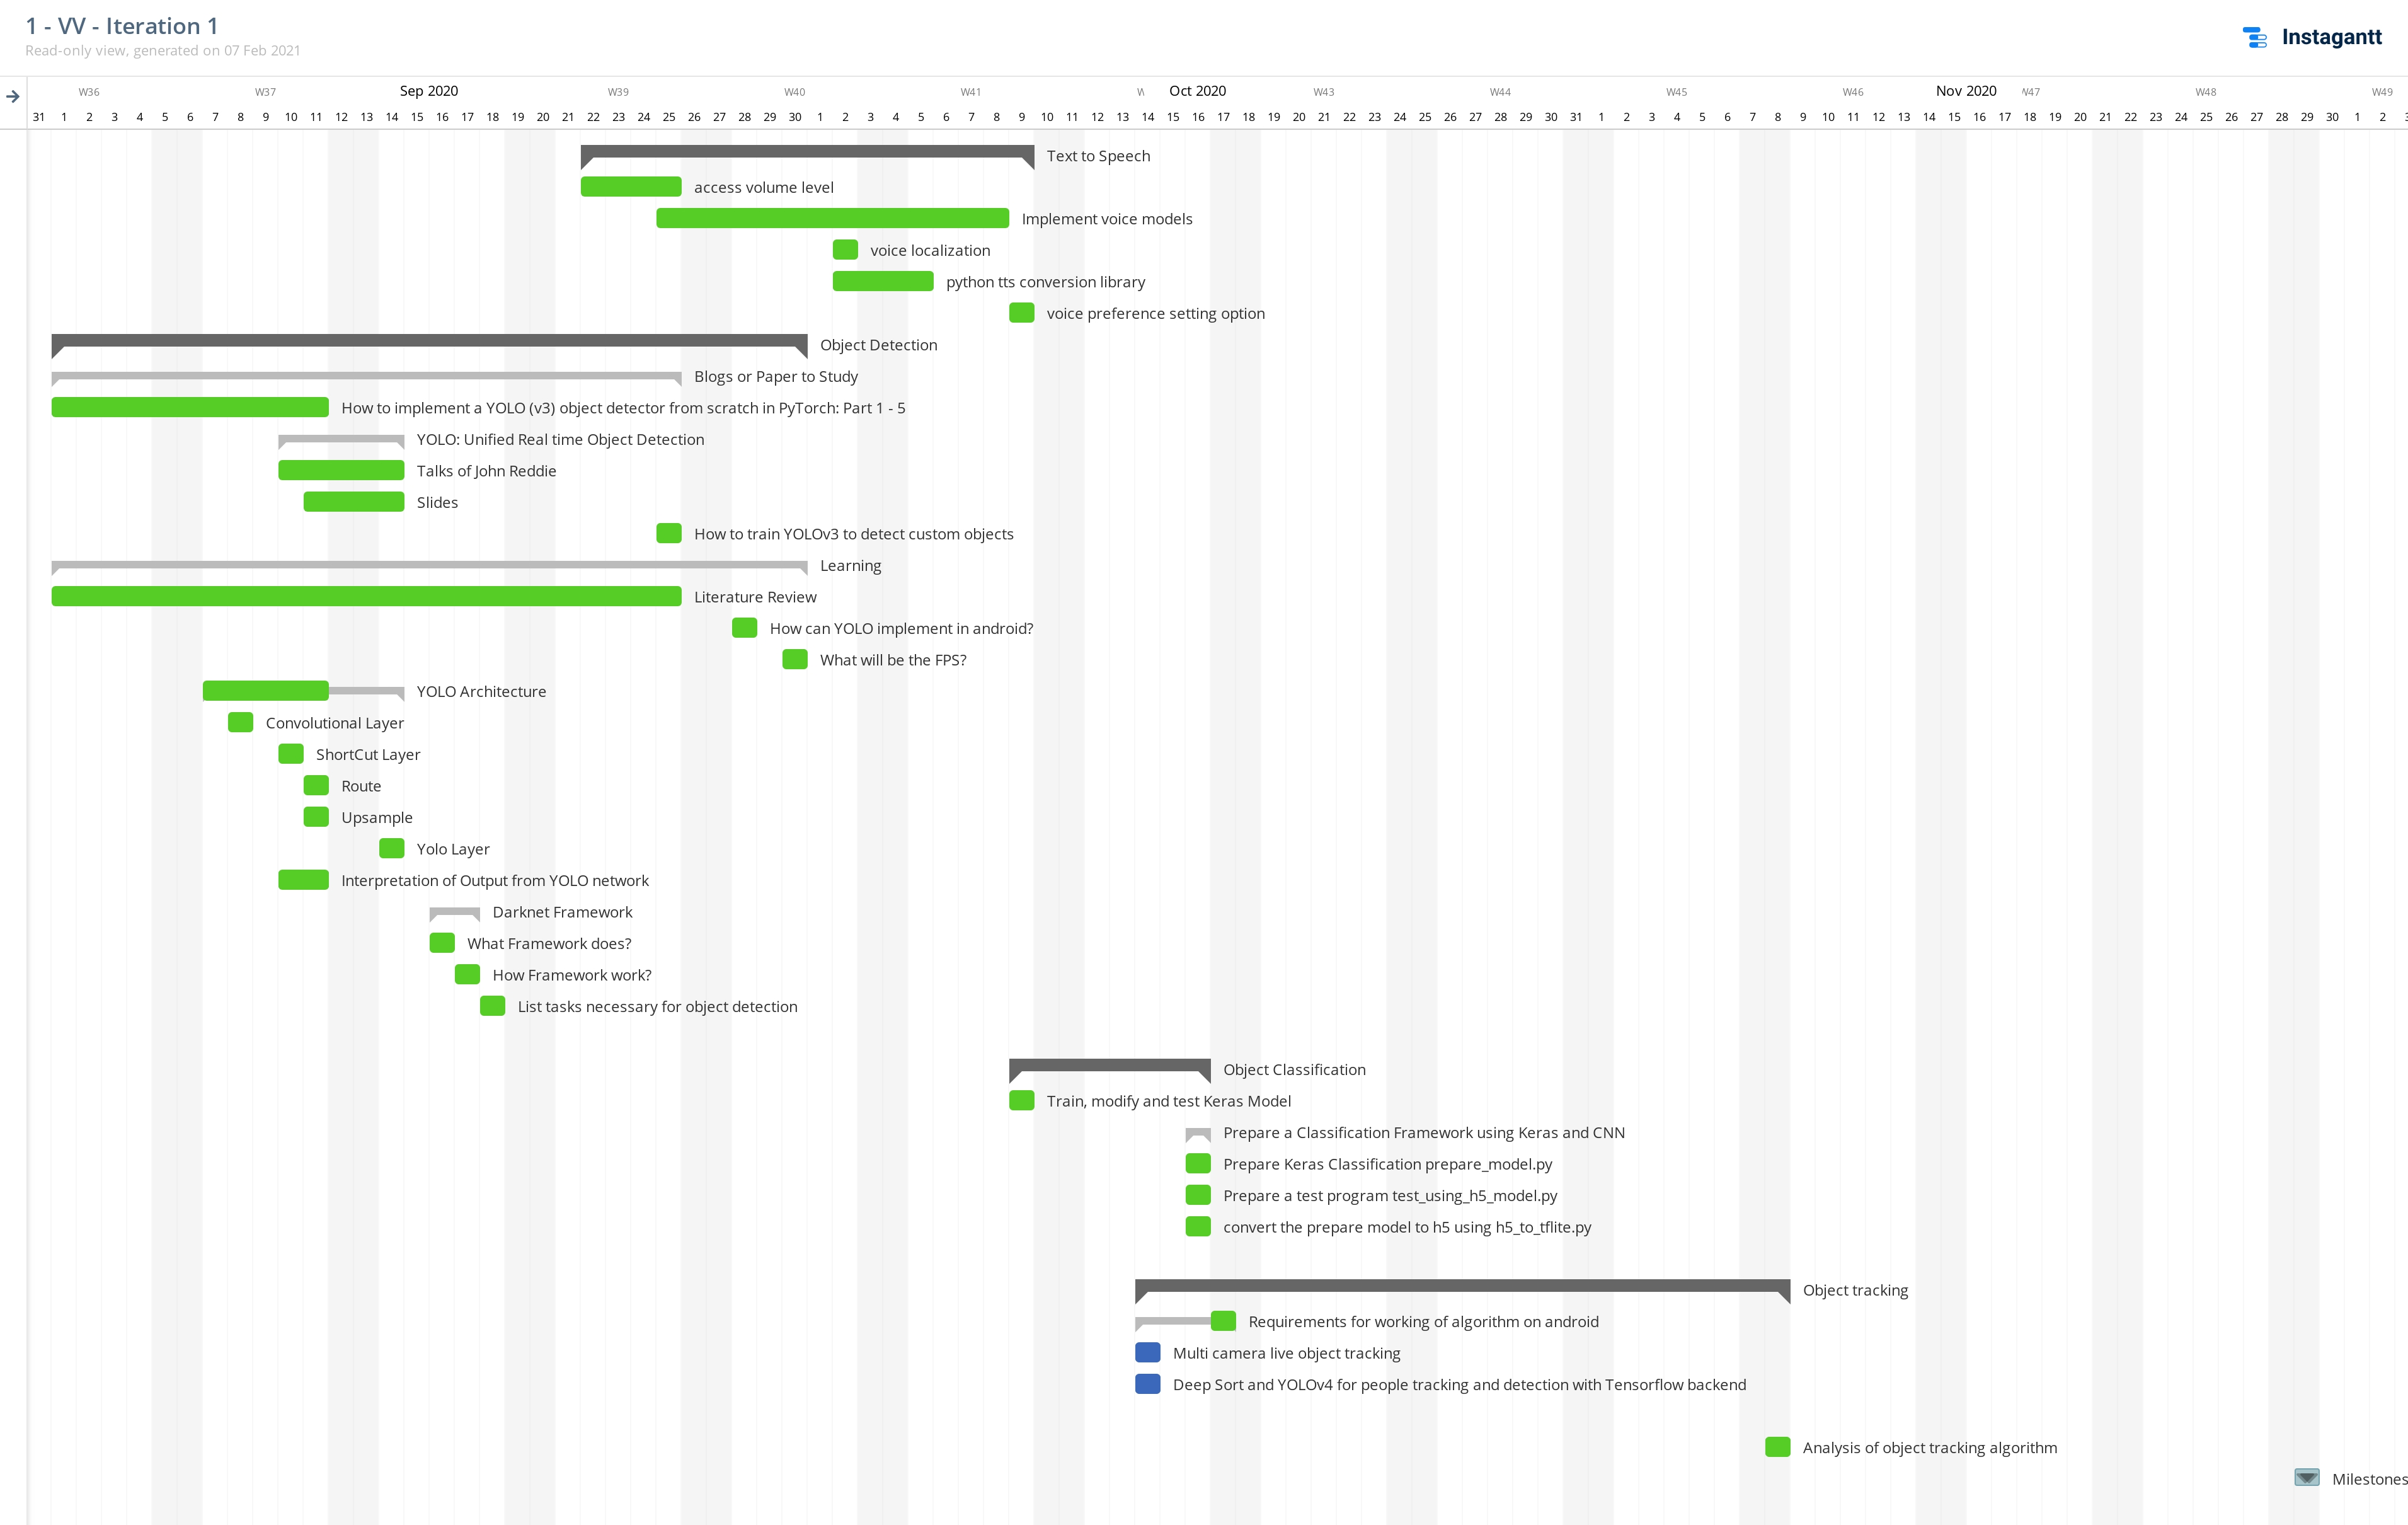
\includegraphics[width=1.0\textwidth]{img/gantt_chart.jpeg}
					\caption{Gantt Chart of project for iteration1 made with Instagantt}    
			\end{figure}
			\section{Assistance for Running the Project}
				\subsection*{How to install CUDA 10.1 with cudnn 7.6.5}
					\subsubsection*{Do Not Install Nvidia Driver}
						During CUDA 10 installation, the driver will be installed. So just go ahead and install CUDA

						\begin{verbatim}
							sudo add-apt-repository ppa:graphics-drivers/ppa
							sudo apt-get update
							sudo apt-get install nvidia-driver-440
						\end{verbatim}
						\textbf{Reboot here, then run below to verify}
						\begin{verbatim}
							nvidia-smi
							dpkg -l | grep nvidia
						\end{verbatim}
					
					\subsubsection*{Install CUDA 10.1}
						Installation Instruction from Nvidia official website:
						
						\begin{verbatim}
							wget https://developer.download.nvidia.com/compute/cuda/repos/ubuntu1804
							/x86_64/cuda-ubuntu1804.pin

							sudo mv cuda-ubuntu1804.pin /etc/apt/preferences.d/cuda-repository-pin-600

							wget http://developer.download.nvidia.com/compute/cuda/10.1/Prod/local_
							installers/cuda-repo-ubuntu1804-10-1-local-10.1.243-418.87.00_1.0-1_amd64.deb

							sudo dpkg -i cuda-repo-ubuntu1804-10-1-local
							-10.1.243-418.87.00_1.0-1_amd64.deb

							sudo apt-key add /var/cuda-repo-10-1-local-10.1.243-418.87.00/7fa2af80.pub

							sudo apt-get update

							sudo apt-get -y install cuda
						\end{verbatim}
						\textbf{Restart Machine}
					
					\subsubsection*{Install cuDNN}
						Goto page \href{https://developer.nvidia.com/rdp/cudnn-download}{https://developer.nvidia.com/rdp/cudnn-download}\\
						\textbf{Download all three .deb: runtime/developer/code sample}

						\begin{verbatim}
							sudo dpkg -i libcudnn7_7.6.5.32-1+cuda10.1_amd64.deb
							sudo dpkg -i libcudnn7-dev_7.6.5.32-1+cuda10.1_amd64.deb
							sudo dpkg -i libcudnn7-doc_7.6.5.32-1+cuda10.1_amd64.deb
						\end{verbatim}

						Now we can verify the cuDNN installation (below is just the official guide, which surprisingly works out of the box):
						\begin{enumerate}
							
							\item Go to the MNIST example code:
								\begin{verbatim}
									cd /usr/src/cudnn_samples_v7/mnistCUDNN/
								\end{verbatim}
							
								\item Compile the MNIST example
								\begin{verbatim}
									sudo make clean && sudo make
								\end{verbatim}
							
								\item Run the MNIST example:
								\begin{verbatim}
									/mnistCUDNN
								\end{verbatim}
								If your installation is successful, you should see 
								\begin{verbatim}
									Test passed!
								\end{verbatim}
								at the end of the output.
						\end{enumerate} 
						\pagebreak
				\subsection*{Deep Sort And YOLO V4}
					\subsubsection*{Clone Git Project}
						\begin{verbatim}
							https://gitlab.com/khwopa1/VV.git
						\end{verbatim}
					\subsubsection*{Installation Required}	
						To run the project, python3.6 or above required and pip3 with latest version 20.X.X\\
						Upgrade the pip3 version to latest
						version\ldots (Required)
						\begin{verbatim}
							sudo -H pip3 install --upgrade pip
						\end{verbatim}
						To run the required libraries run the install.sh file as:
						\begin{verbatim}
							./install.sh
						\end{verbatim}				
					\subsubsection*{Inclusion needed (Optional since file is already converted and stored in model\_data)}
						Download and add yolov4.weights file in model\_data folder,
						then run 
						\begin{verbatim}
							python3 convert.py
						\end{verbatim}
						This will convert the yolov4 weights file to keras model (.h5 file) The keras model will save in the model\_data directory..
					\subsubsection*{Inference}
						\begin{verbatim}
							python3 main.py
						\end{verbatim}
						Change video name on line 59 in main.py
						\begin{verbatim}
							self.filename = `[filename]'
						\end{verbatim}
						\pagebreak
				\subsection*{Mot-ground-truth}
					\subsubsection*{How to use?}
						\begin{verbatim}
							python3 main.py --data [directory containing images] --dest [filename 
							to store result]
						\end{verbatim}
					\subsubsection*{Preprocessing}
						For this, the image must be stored in a directory and name it like 1.jpg, 2.jpg, \ldots and do not brake in naming from 1,2,3\ldots ..
					\subsubsection*{During Run time}
						Image will open\ldots Be careful don't click on image,
						\begin{enumerate} 
							\item The First image will open with name 1.jpg.
							\item There select the rectangle box:
								\begin{itemize}
									\item First pick the first point.
									\item Pick the second point.
									\item Then, you will be ask to input track id, there enter the track id.
								\end{itemize}
							\item Repeat the 2. step for other object in that image also.
							\item Press ESC to get next image.
							\item Repeat the step 2 and 3.
						\end{enumerate}
					\subsubsection*{MOT-evaluation}
						How to use? 
						\begin{verbatim}
							python3 evaluate_tracking.py --seqmap [Path to seqmap file] 
							--track [Path to Tracking result directory] 
							--gt [Path to Ground-truth annotation directory]
						\end{verbatim}
						
					\subsubsection*{Preprocessing}
						The sequence map must be update with the required directory name. Generally the directory name will match with the video file name.
